\chapter{A Precise Half-Wave Rectifier: Part I}


\section{Objectives}
\begin{itemize}
    \item To verify one precise full-wave rectifier
\end{itemize}

\section{Materials}
\begin{itemize}
    \item Breadboard
    \item DC power supply
    \item Digital Multi-Meter
    \item \hyperref[1N4148]{Diode (1N4148)}
    \item Function Generator
    \item \hyperref[LM741_1]{Op.Amp. (LM741)}
    \item Oscilloscope
    \item Resistors
\end{itemize}

\section{Introduction}
    \subsection{Precise Rectifier}
        \begin{itemize}
            \item \textbf{Precise Rectifier}\par
                With the help of the operational amplifier, the Precise Rectifier can handle the input signal that need to rectify with less power.\par
                Usually the input voltage flew into the circuit is lower than the build-in voltage of the normal diodes. Then the operational amplifier will amplify the signal and make it able to across the diodes reaching the aim of rectifying.
        \end{itemize}
        
    \subsection{Circuit Diagram}
        \begin{figure}[h]
            \centering
            \includegraphics[width=0.7\linewidth]{Lab13/Lab13.drawio.png}
            \caption{Circuit Diagram}
            \label{l13f}
        \end{figure}
        \FloatBarrier

\section{Detailed Procedures}
    \subsection{Analyzation}
    First, we analyze the relationship between $V_i$ and $V_o$ in the circuits.\par
    \begin{itemize}
        \item $V_i > 0, D_1~\text{on}, D_2~\text{off}$\par
            \begin{equation}
                \begin{cases}
                    V_1=V_2=0\\
                    V_3=V_1-V_\gamma=-V_\gamma\\
                    V_4=V_5=0\\
                    \frac{V_i-0}{20k} = \frac{0-V_o}{20k}\\
                \end{cases}
                \label{l13eq1}
            \end{equation}
            From Equation.\ref{l13eq1} and given data, we can obtain\par
            \begin{equation*}
                \begin{cases}
                    V_o=-V_i\\
                    V_1=V_2=0\\
                    V_3=-V_\gamma\\
                    V_4=V_5=0\\
                \end{cases}
            \end{equation*}
            
        \item $V_i < 0, D_1~\text{off}, D_2~\text{on}$
            \begin{equation}
                \begin{cases}
                    V_1=V_2=0\\
                    \frac{V_i-0}{10k}=\frac{0-V_4}{10k}\\
                    V_4=-V_i\\
                    V_5=0\\
                    V_3=-V_i+V_\gamma\\
                    \frac{-V_i-0}{10k}+\frac{V_i-0}{20k}=-\frac{0-V_o}{20k}\\
                \end{cases}
                \label{l13eq2}
            \end{equation}
            From Equation.\ref{l13eq2} and given data, we can obtain\par
            \begin{equation*}
                \begin{cases}
                V_o=V_i\\
                V_1=V_2=0\\
                V_3=-V_i+V_\gamma\\
                V_4=-V_i\\
                V_5=0\\
                \end{cases}
            \end{equation*}
    \end{itemize}

    \subsection{Procedures}
    Construct the circuit as Fig.\ref{l13f} with supply voltages at $\pm$10V.
    \subsubsection{AC}
    Then we used oscilloscope to observe the waveform with $V_i$ as sinusoidal signal input with a fixed frequency of 200 Hz under different amplitude voltages:\par
        \begin{figure}[h]
            \centering
            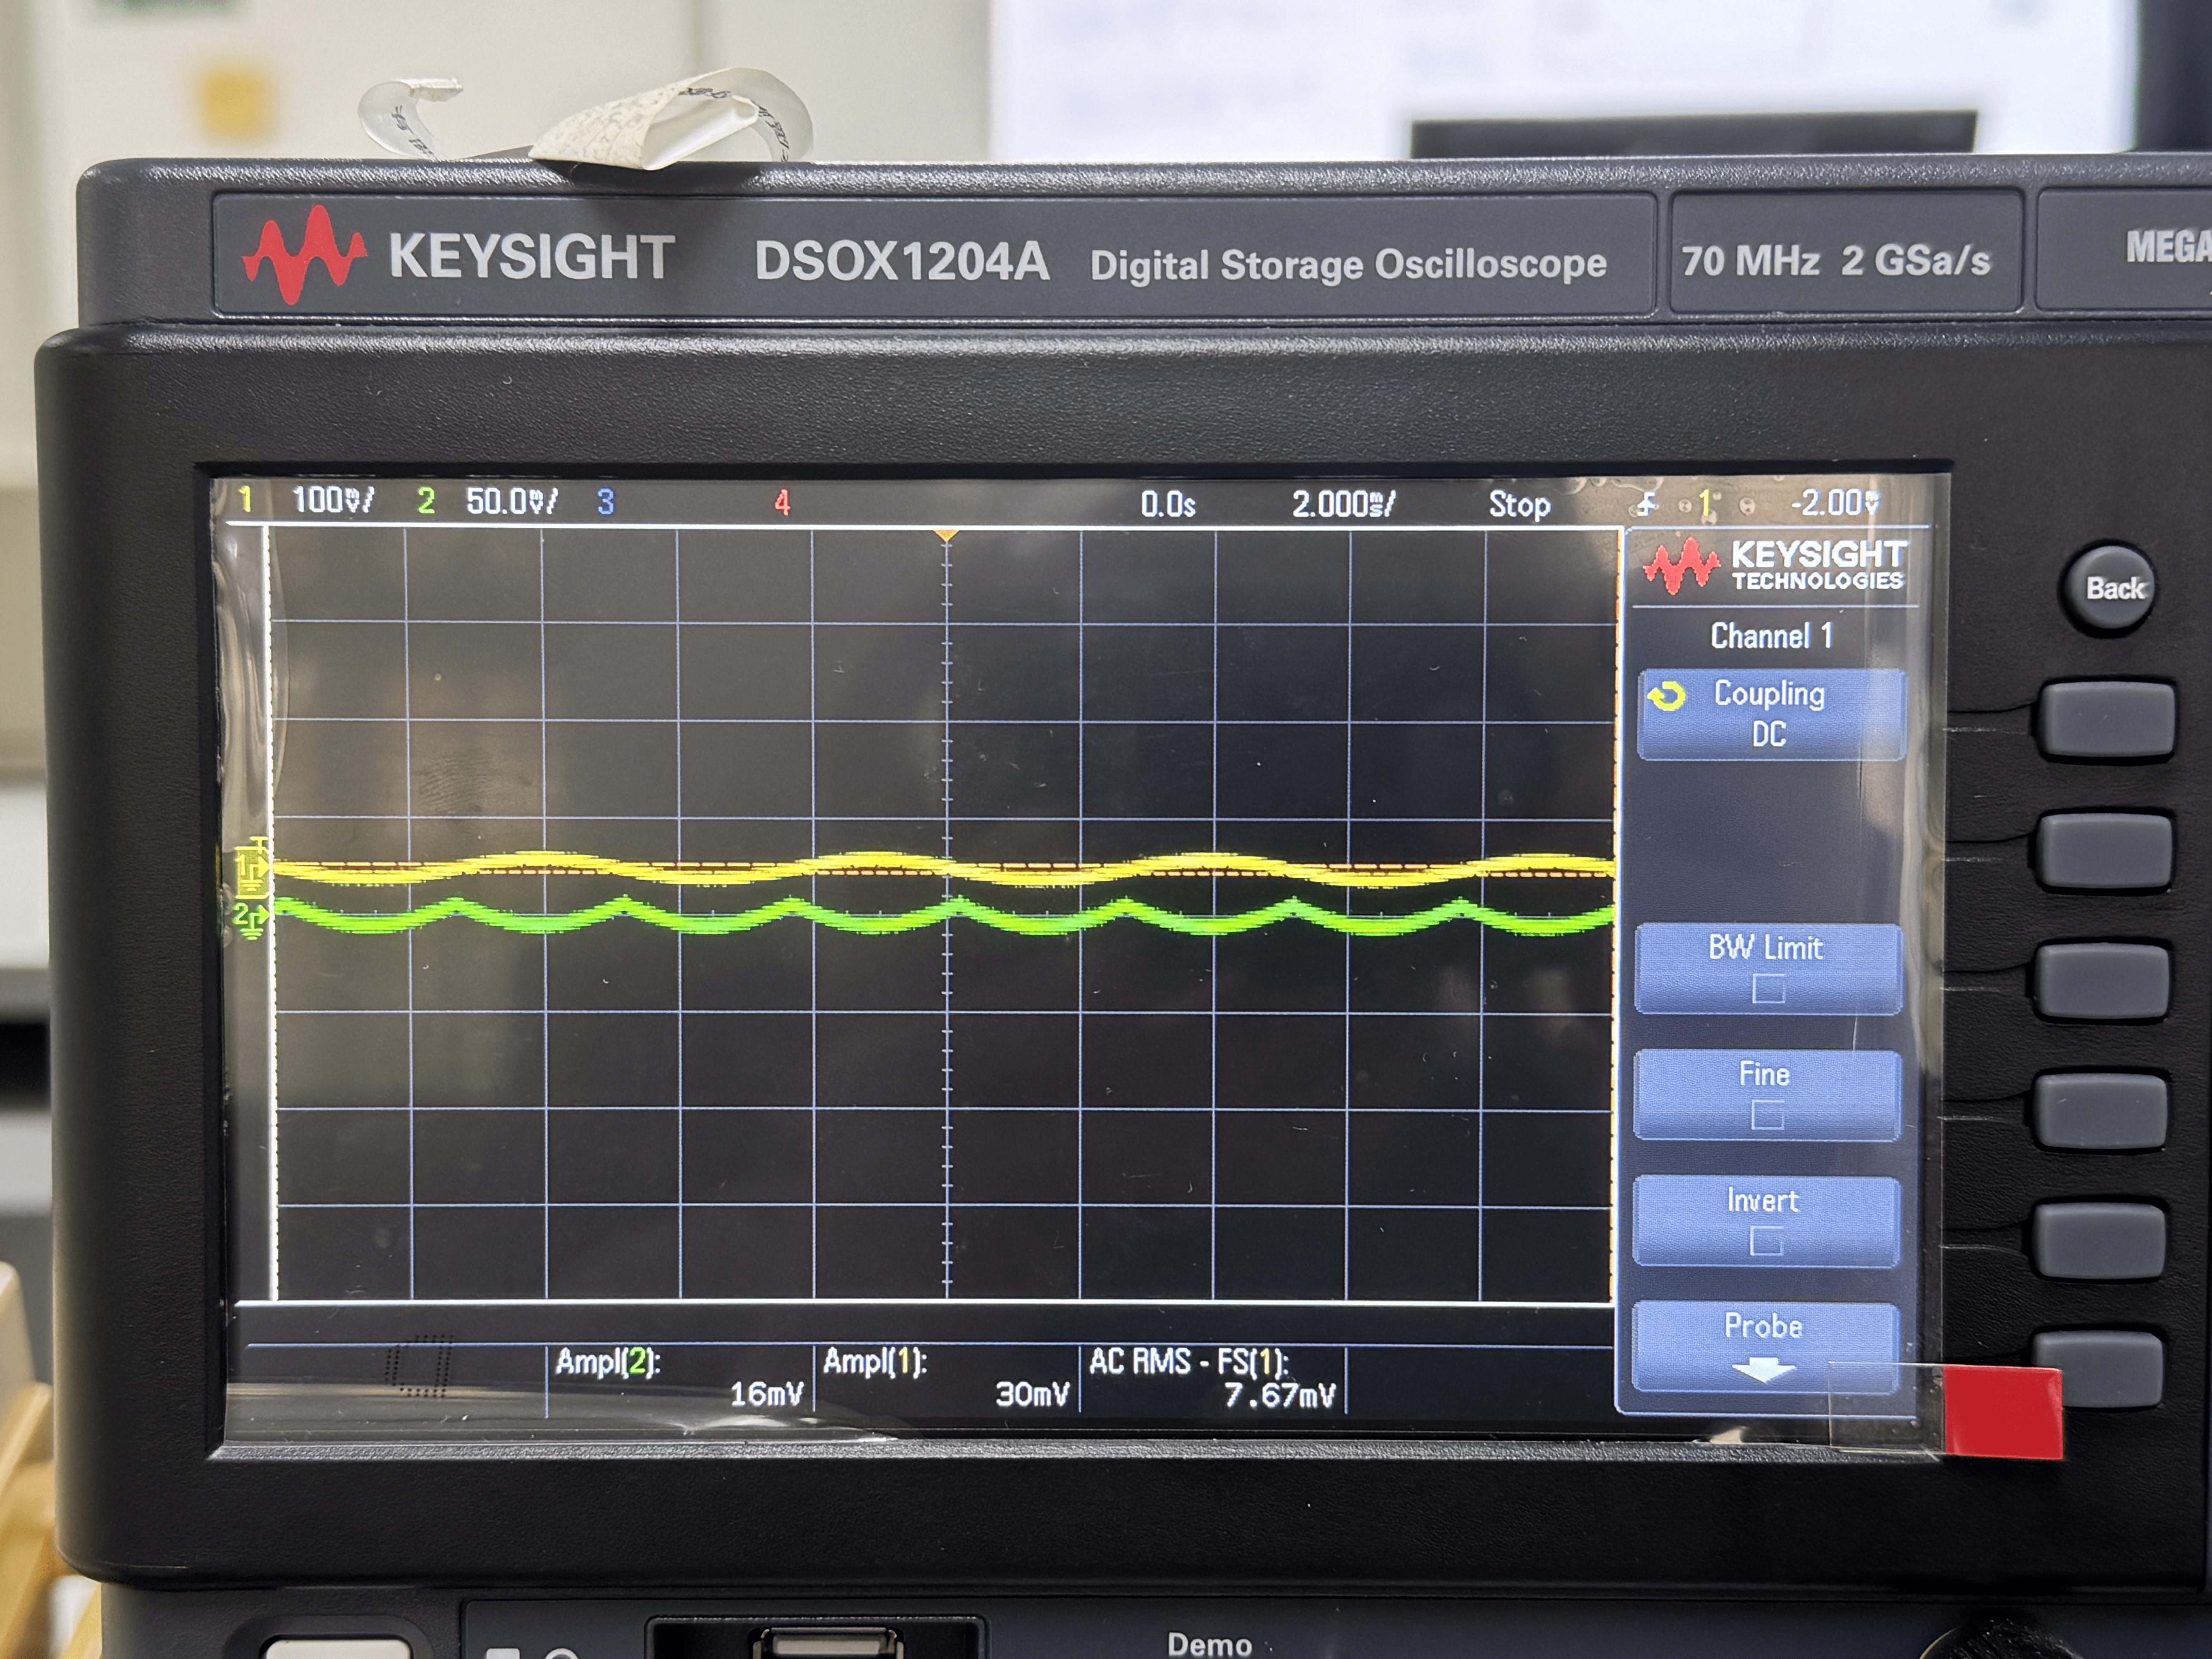
\includegraphics[width=0.5\linewidth]{Lab13/Images/13_0-1v.jpg}
            \caption{$V_i=0.1V$}
            \label{l13vi01v}
        \end{figure}
        \FloatBarrier
        \begin{figure}[h]
            \centering
            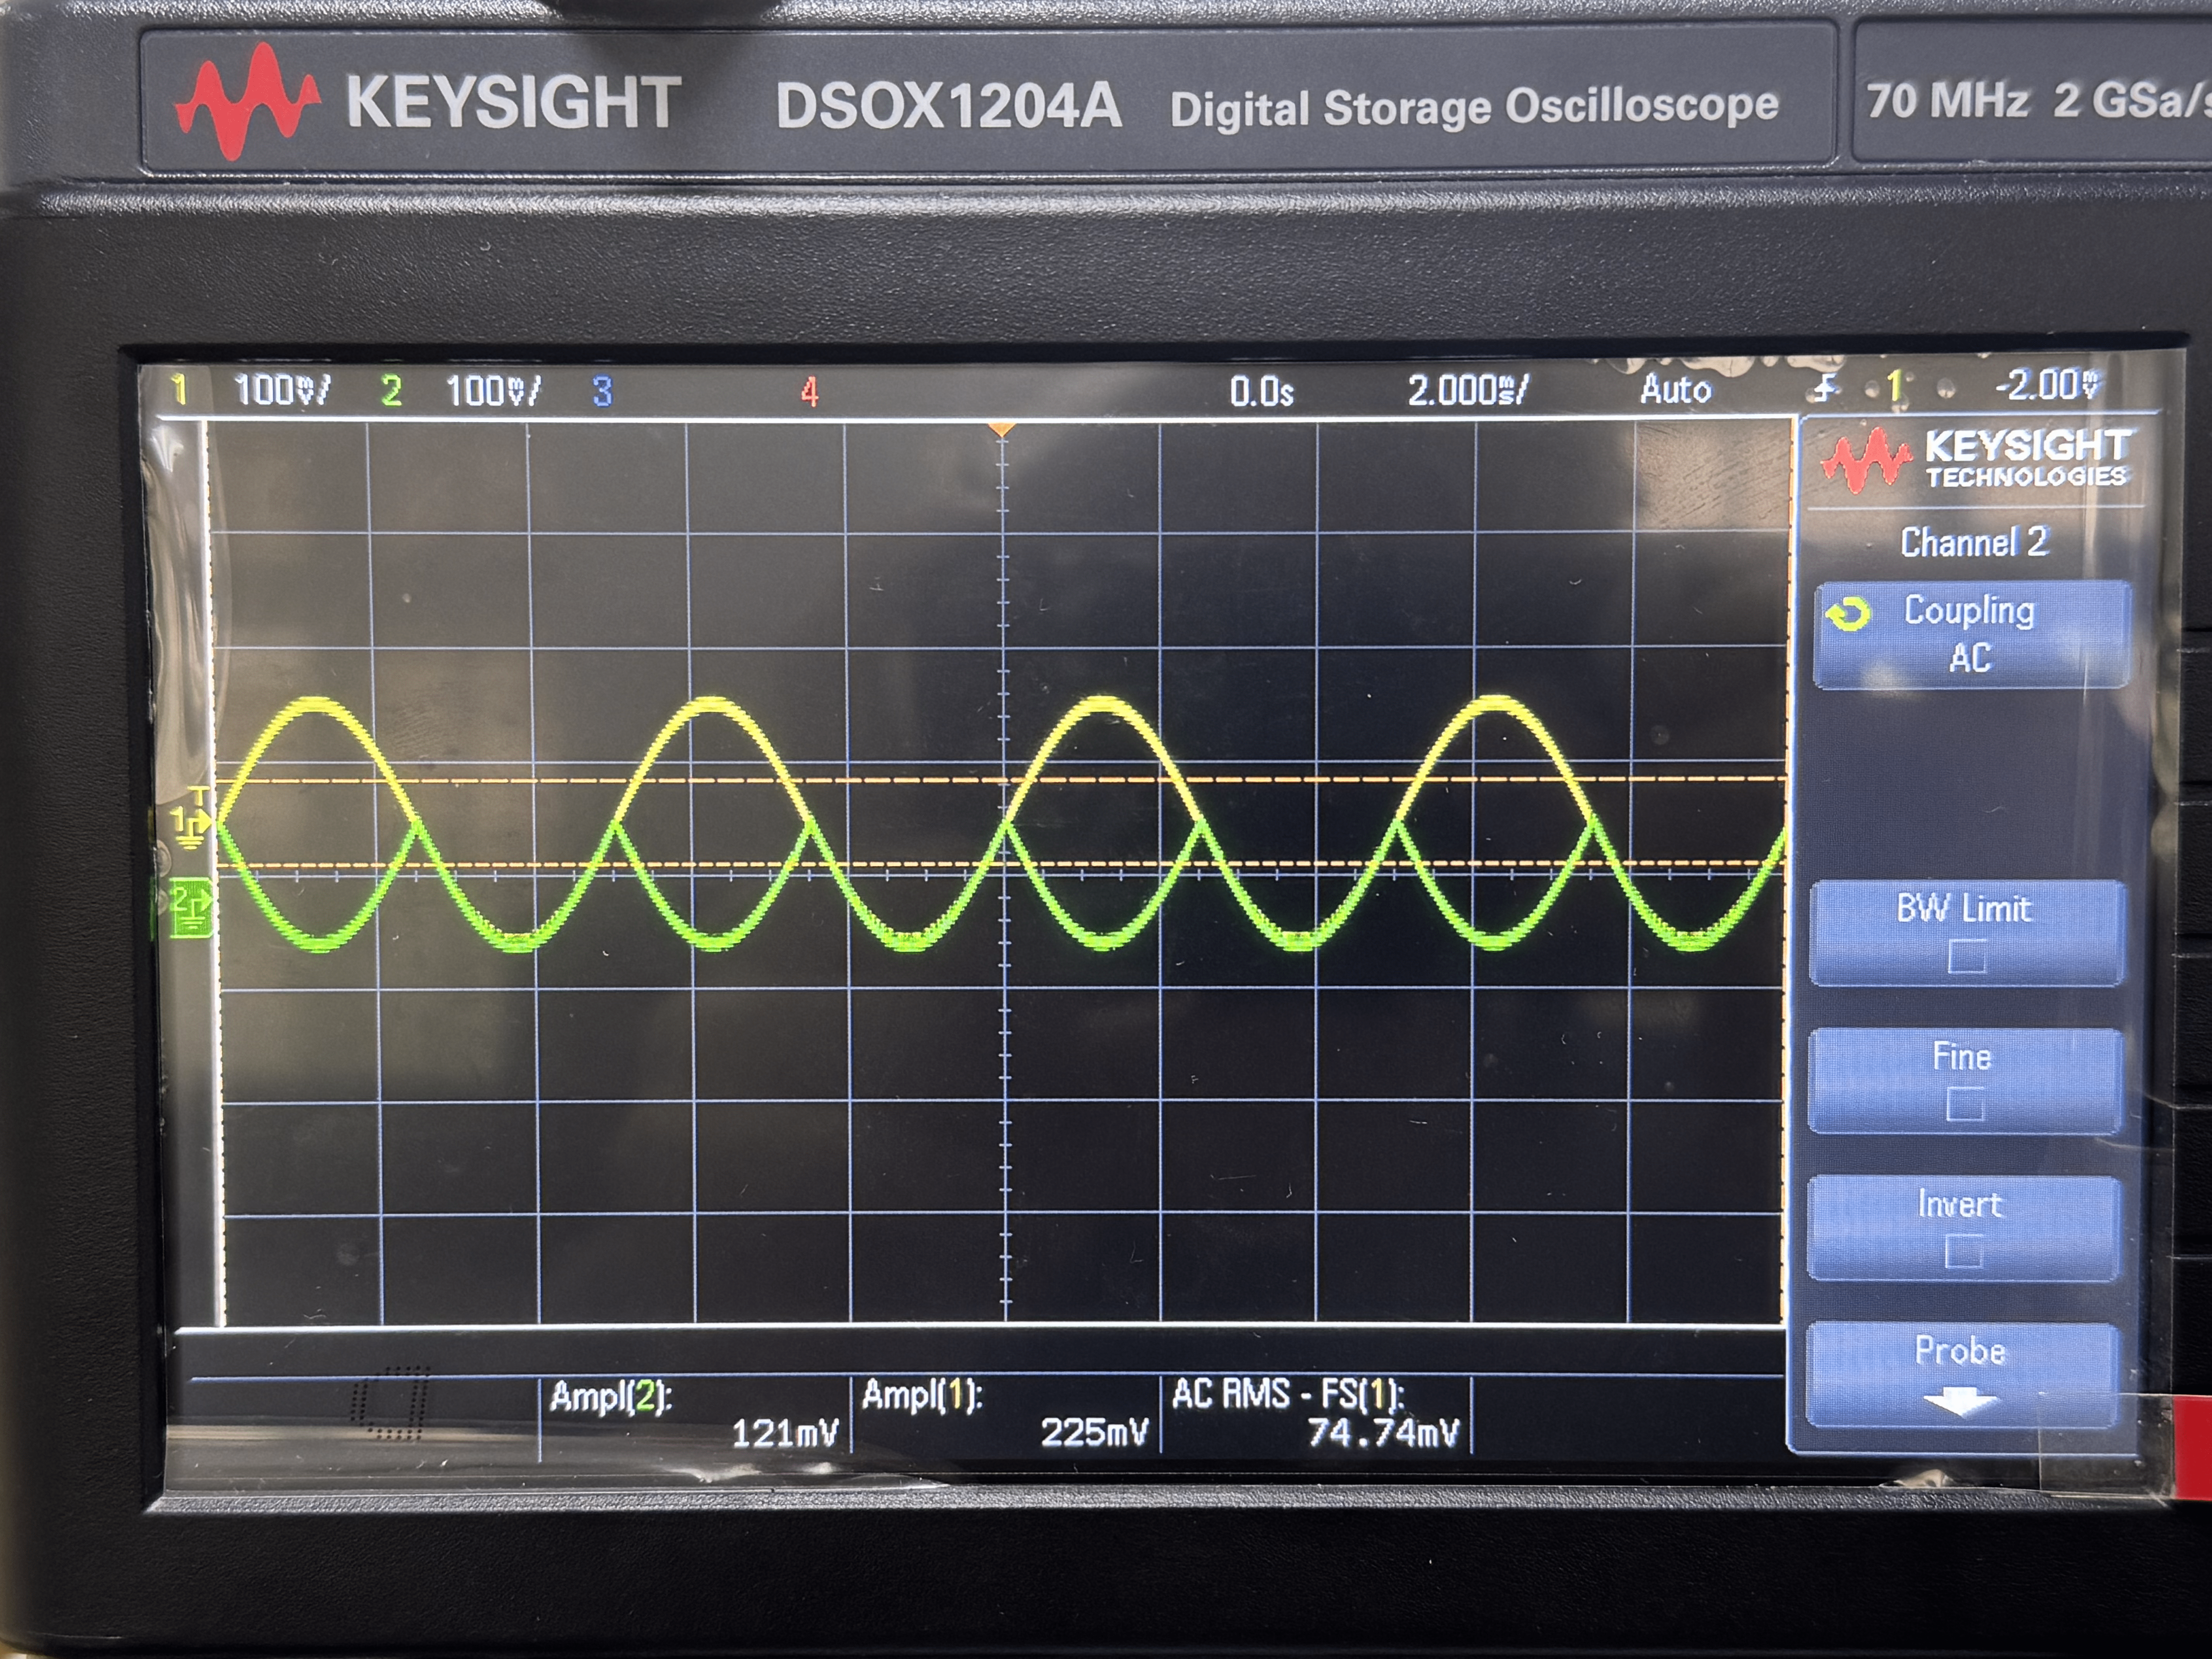
\includegraphics[width=0.5\linewidth]{Lab13/Images/13_1v.jpg}
            \caption{$V_i=1V$}
            \label{l13vi1v}
        \end{figure}
        \FloatBarrier
        \begin{figure}[h]
            \centering
            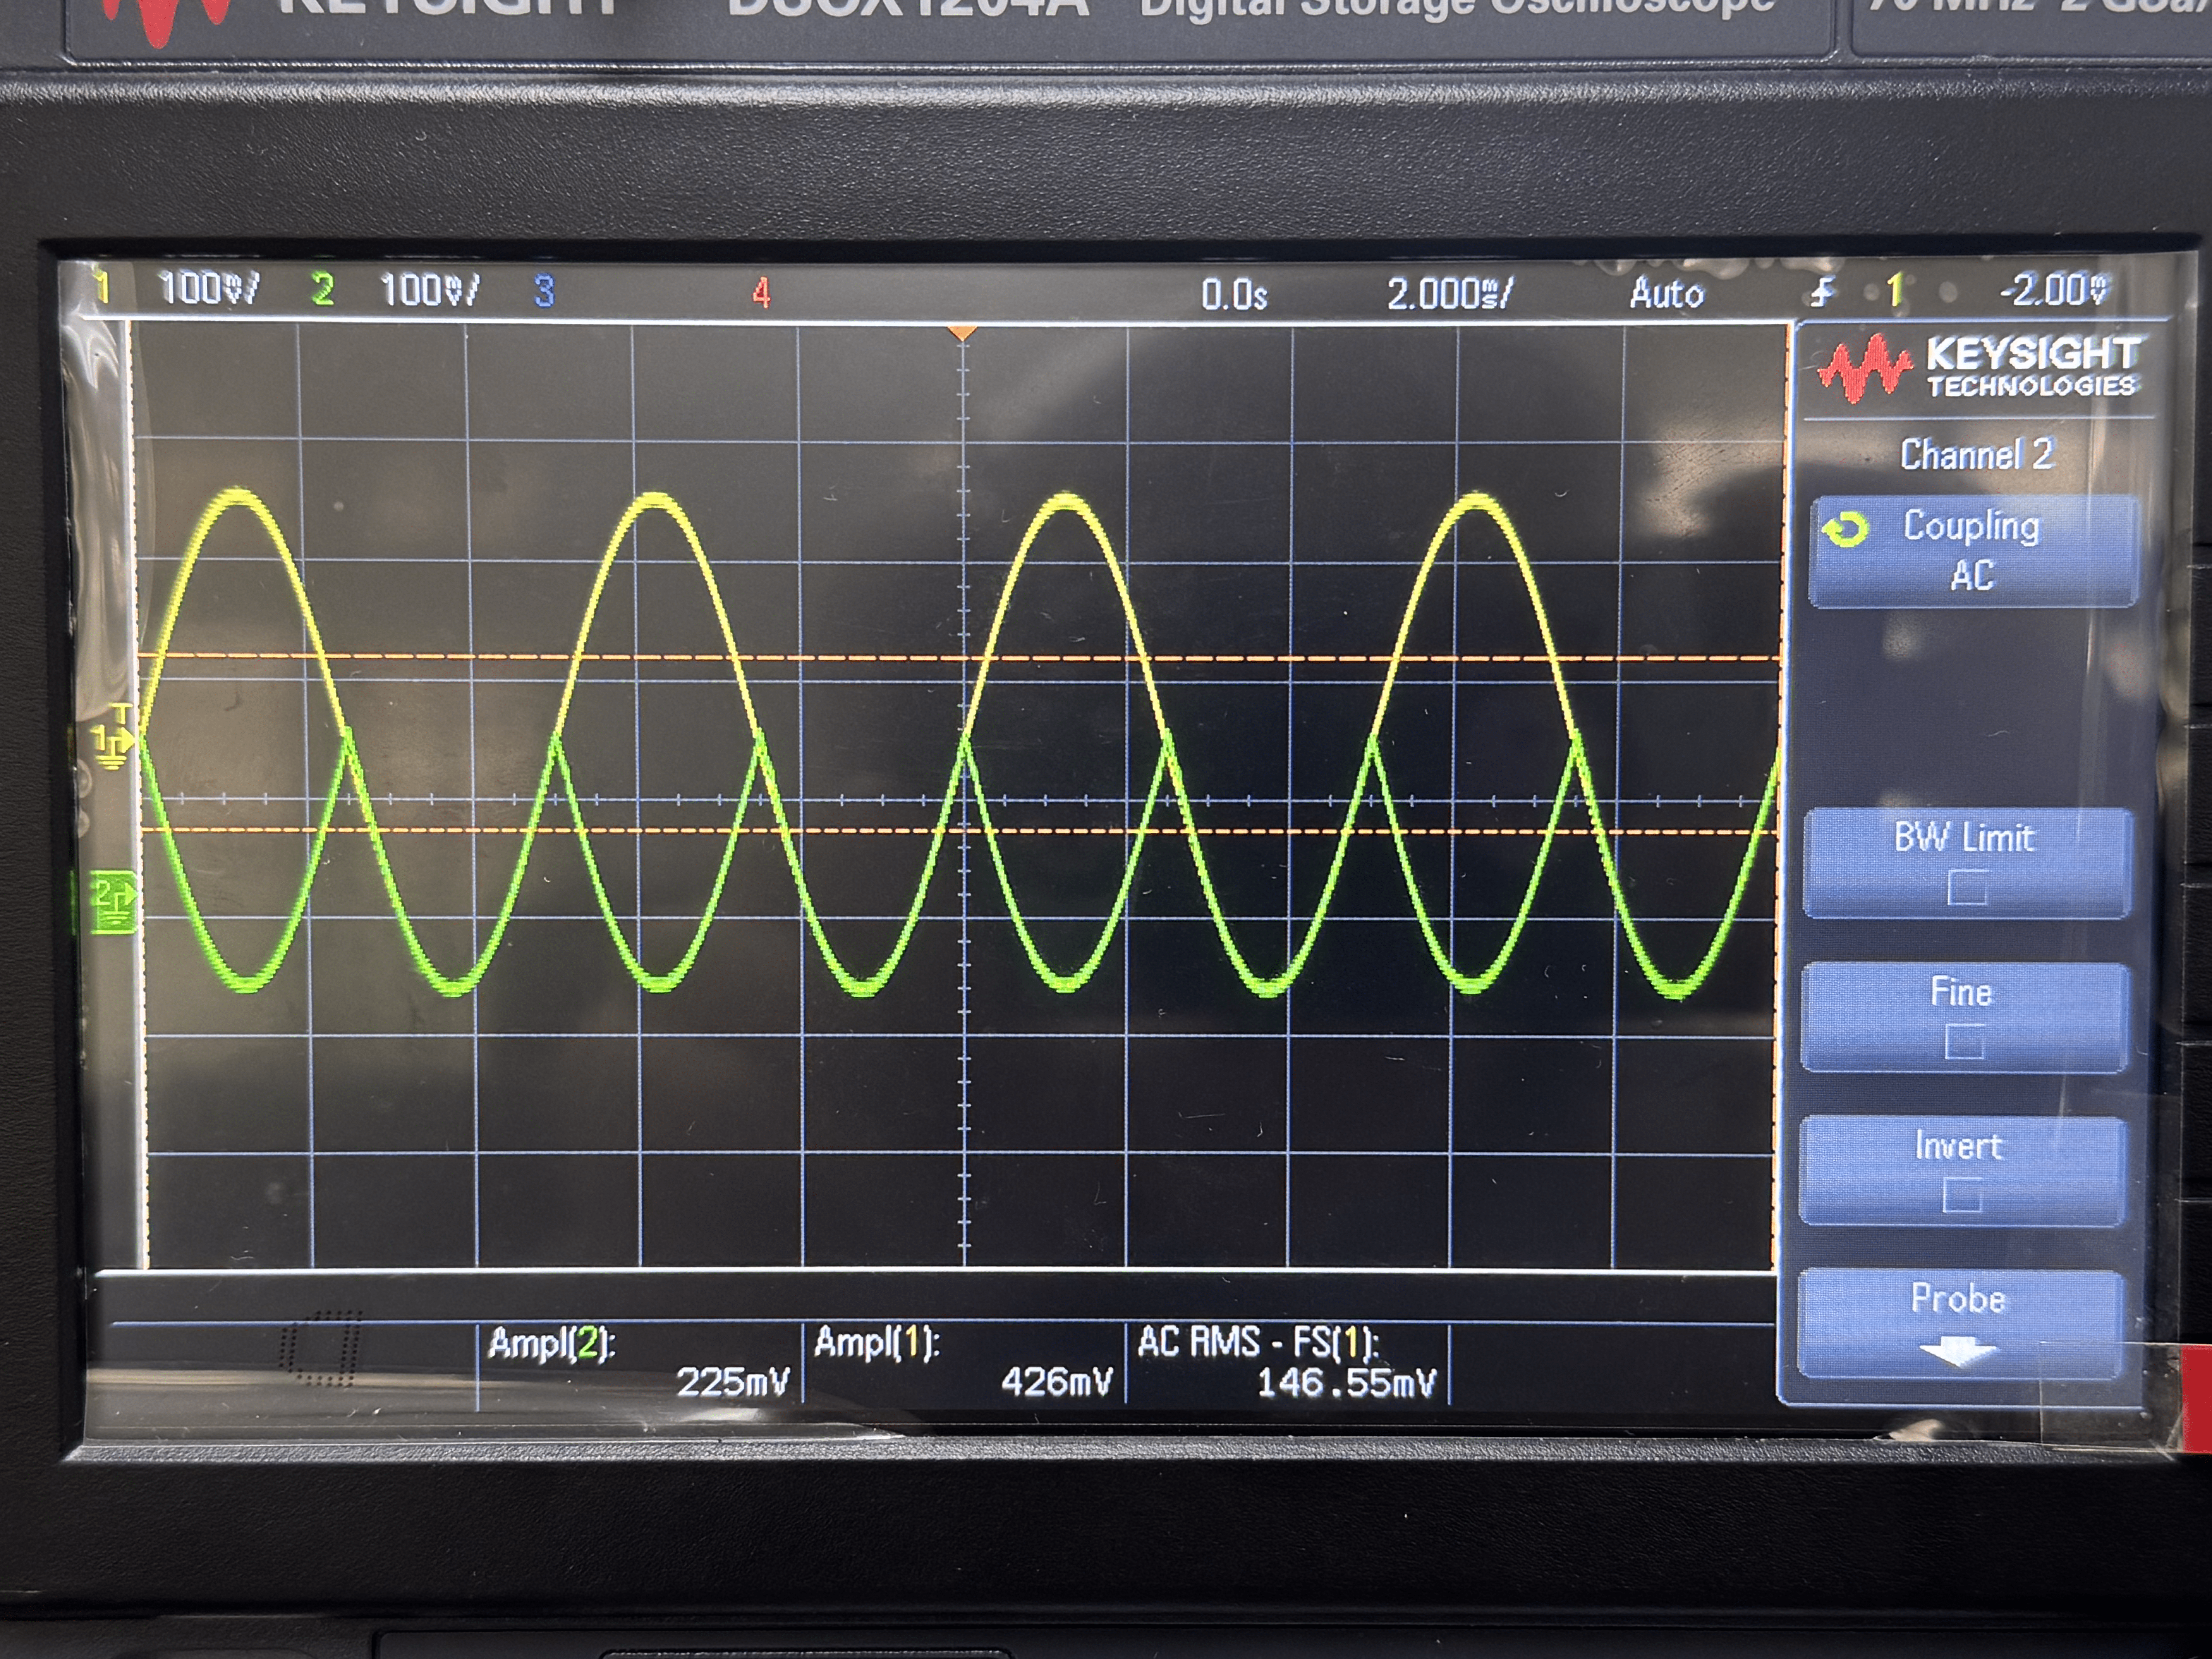
\includegraphics[width=0.5\linewidth]{Lab13/Images/13_2v.jpg}
            \caption{$V_i=2V$}
            \label{l13vi2v}
        \end{figure}
        \FloatBarrier
        \begin{figure}[h]
            \centering
            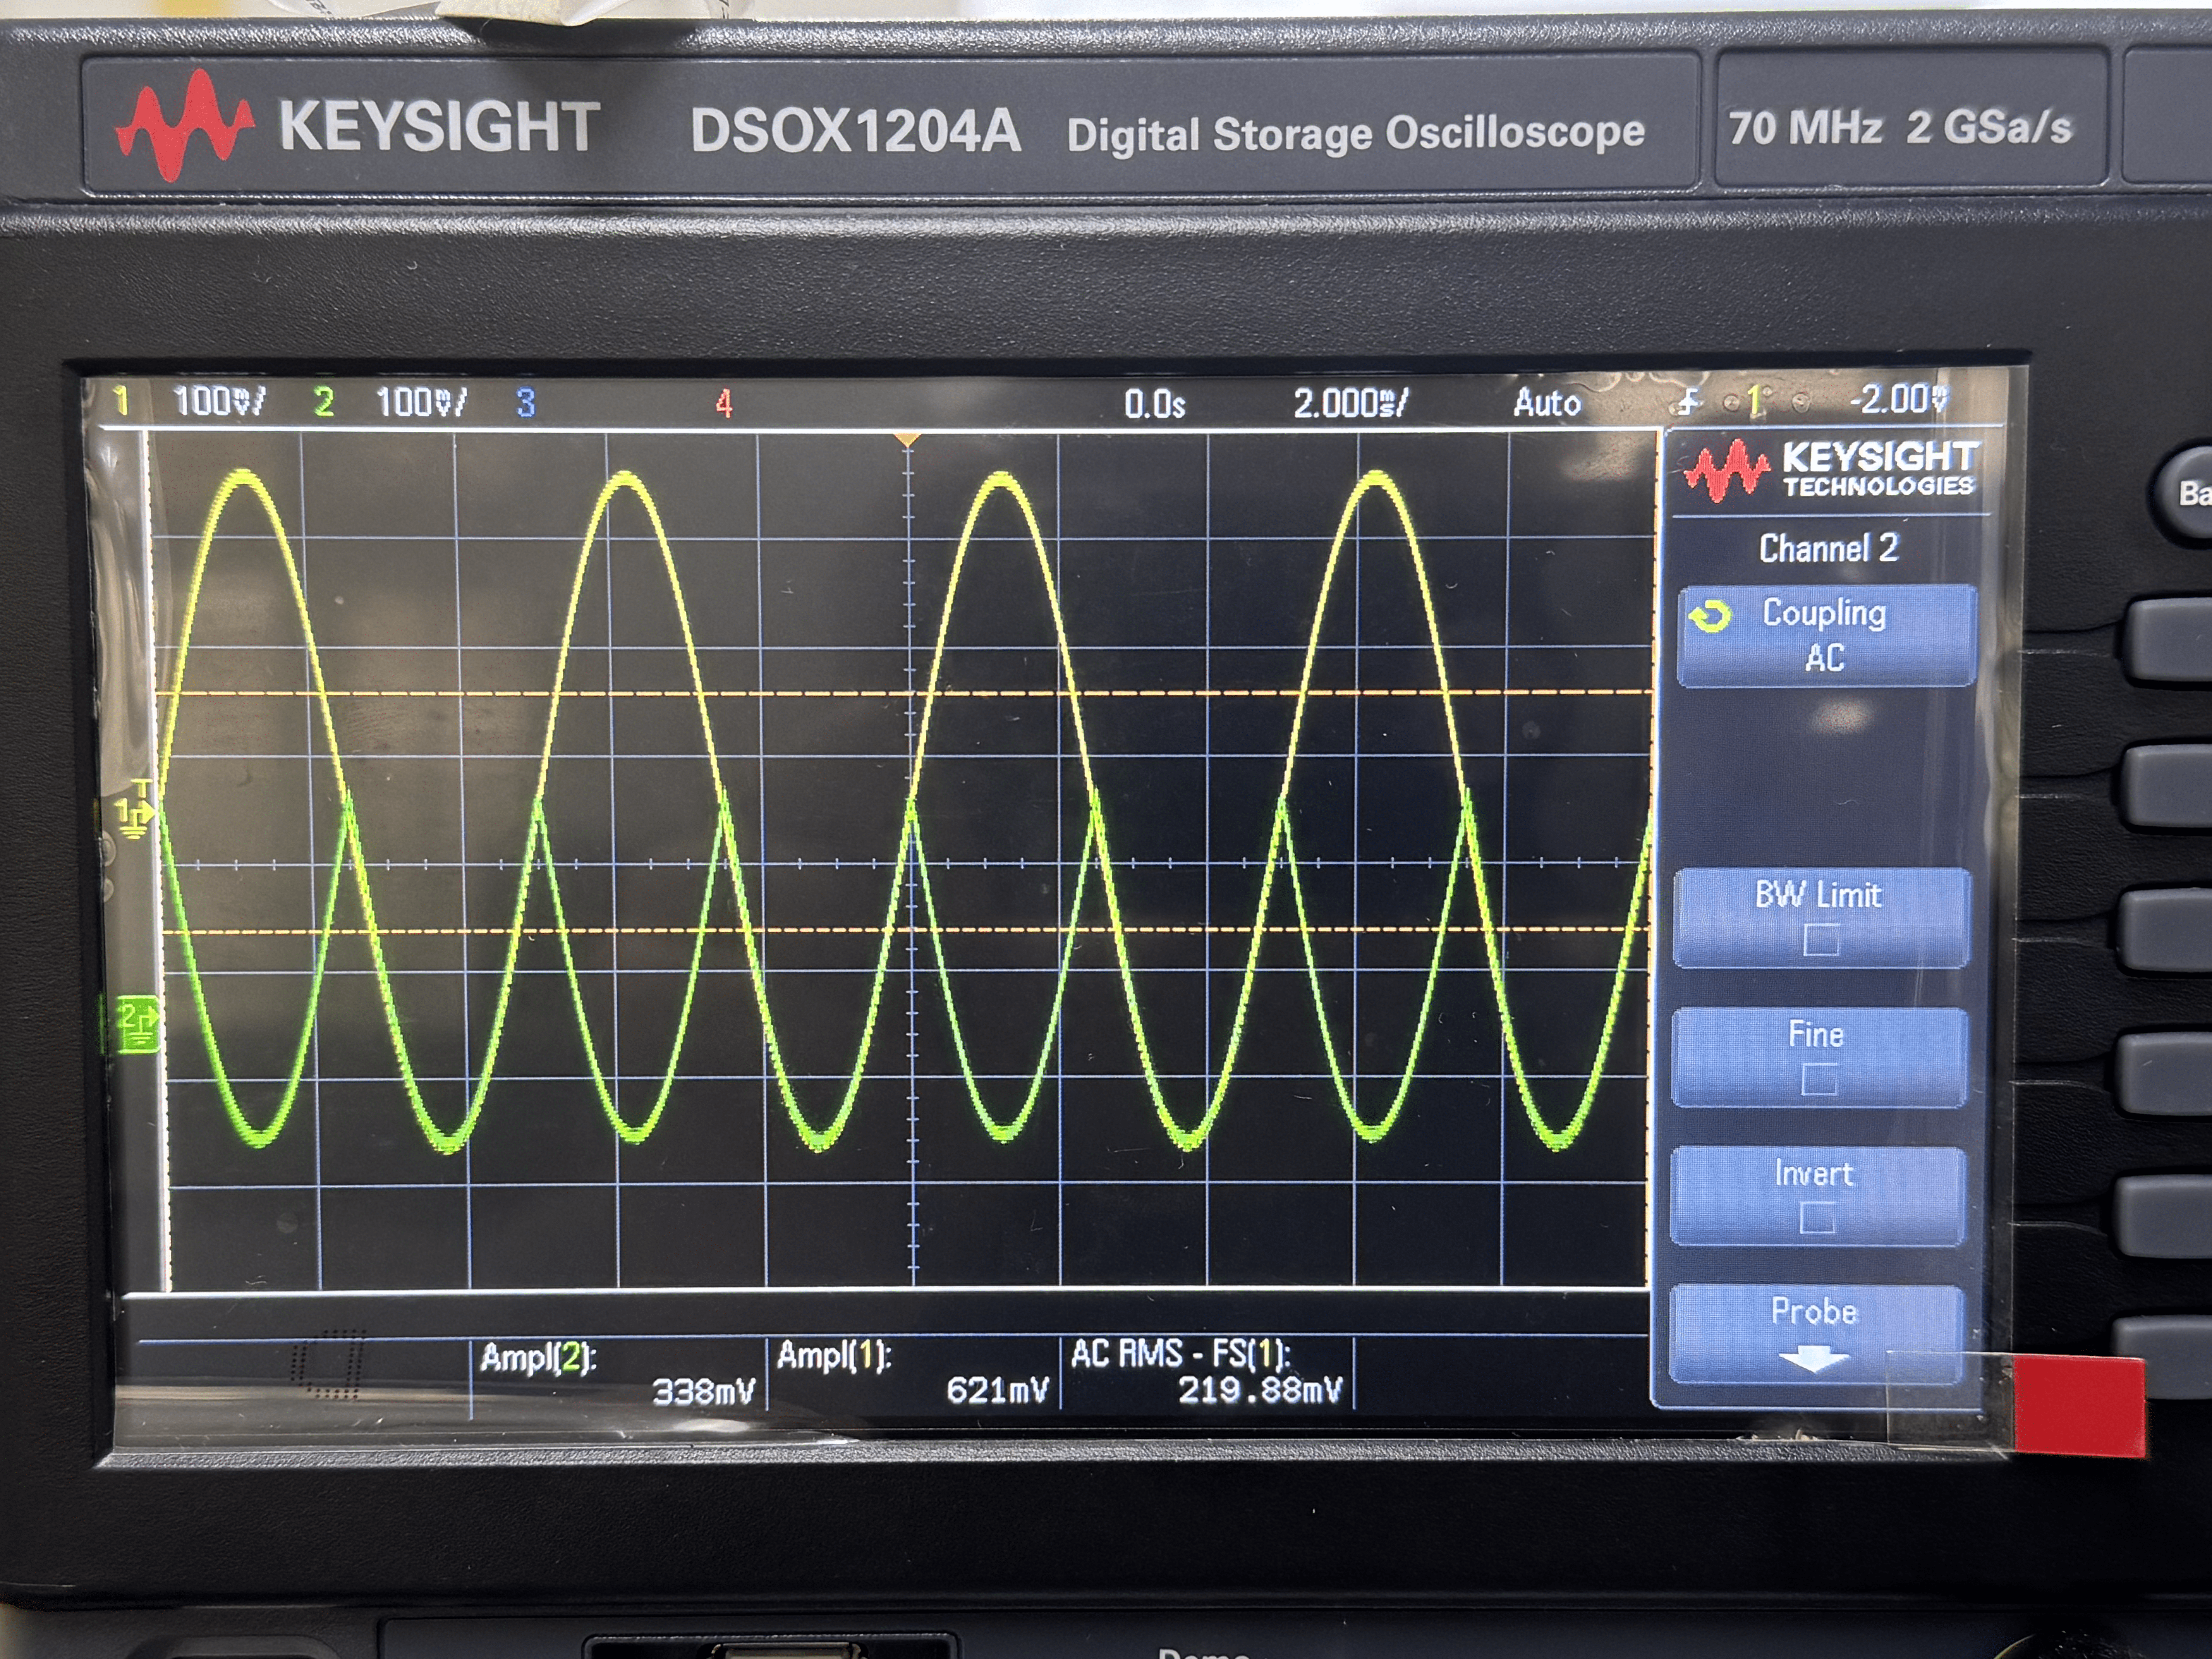
\includegraphics[width=0.5\linewidth]{Lab13/Images/13_3v.jpg}
            \caption{$V_i=3V$}
            \label{l13vi3v}
        \end{figure}
        \FloatBarrier
        \begin{figure}[h]
            \centering
            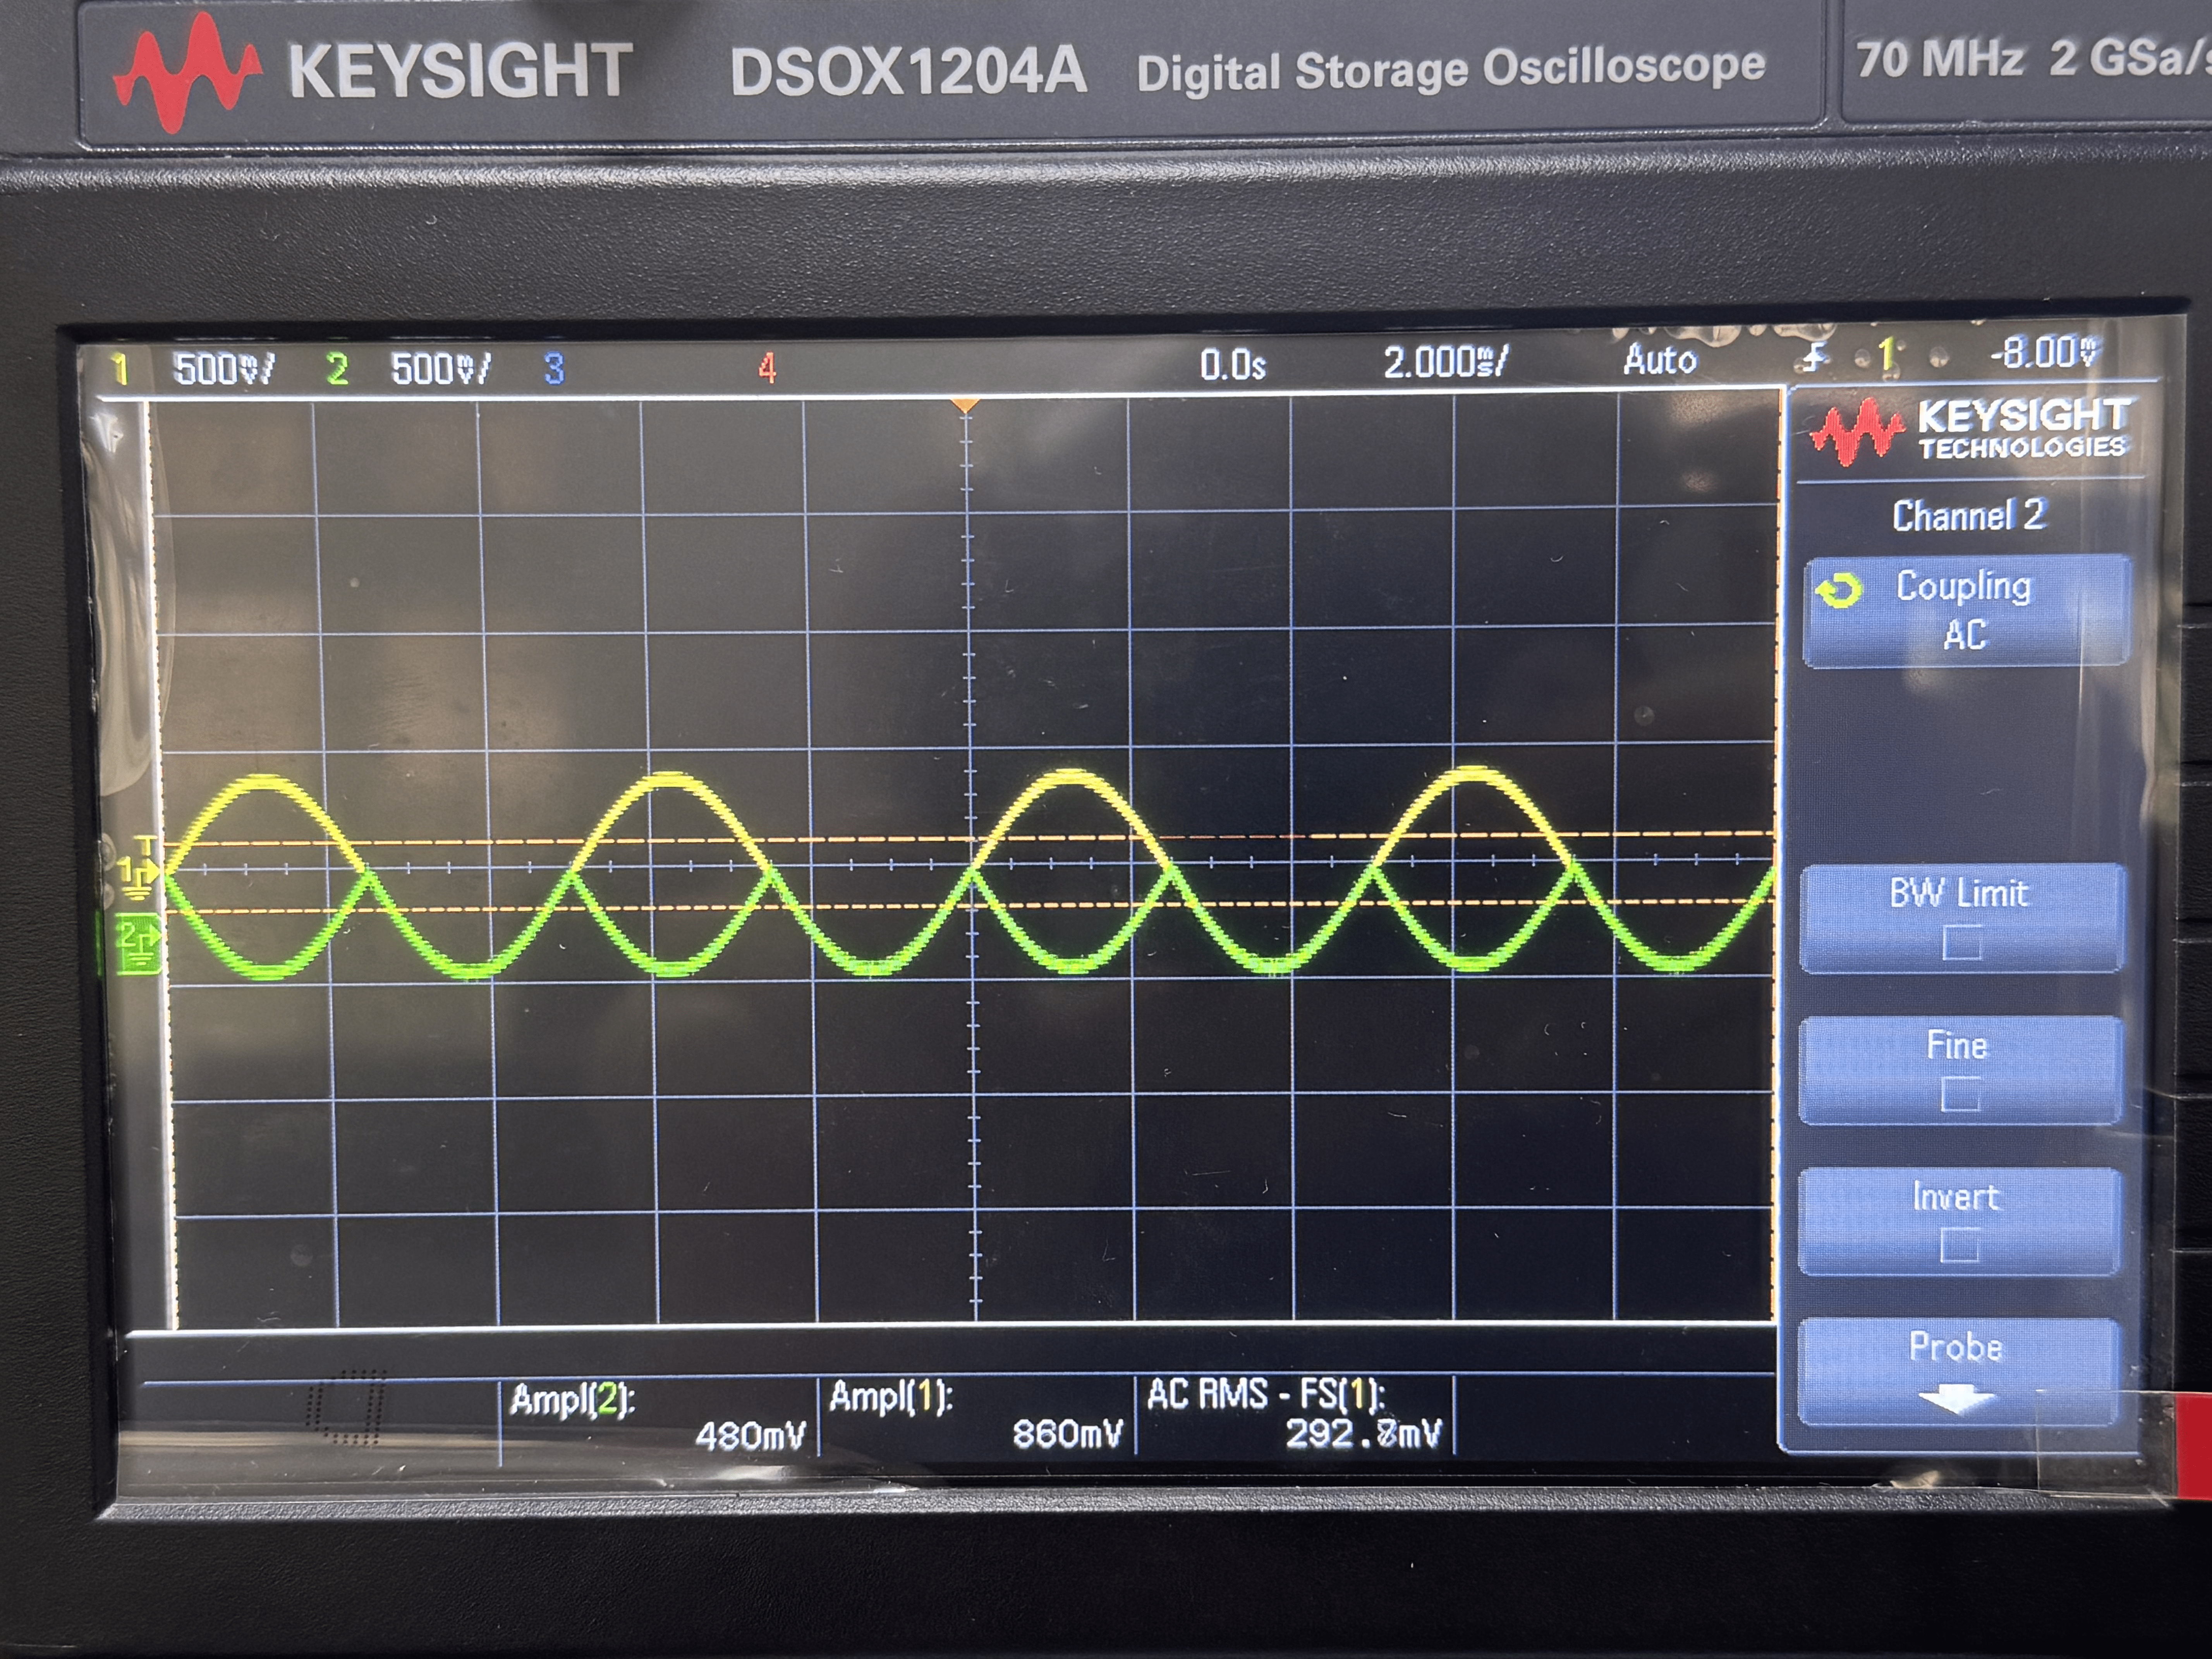
\includegraphics[width=0.5\linewidth]{Lab13/Images/13_4v.jpg}
            \caption{$V_i=4V$}
            \label{l13vi4v}
        \end{figure}
        \FloatBarrier
        \begin{figure}[h]
            \centering
            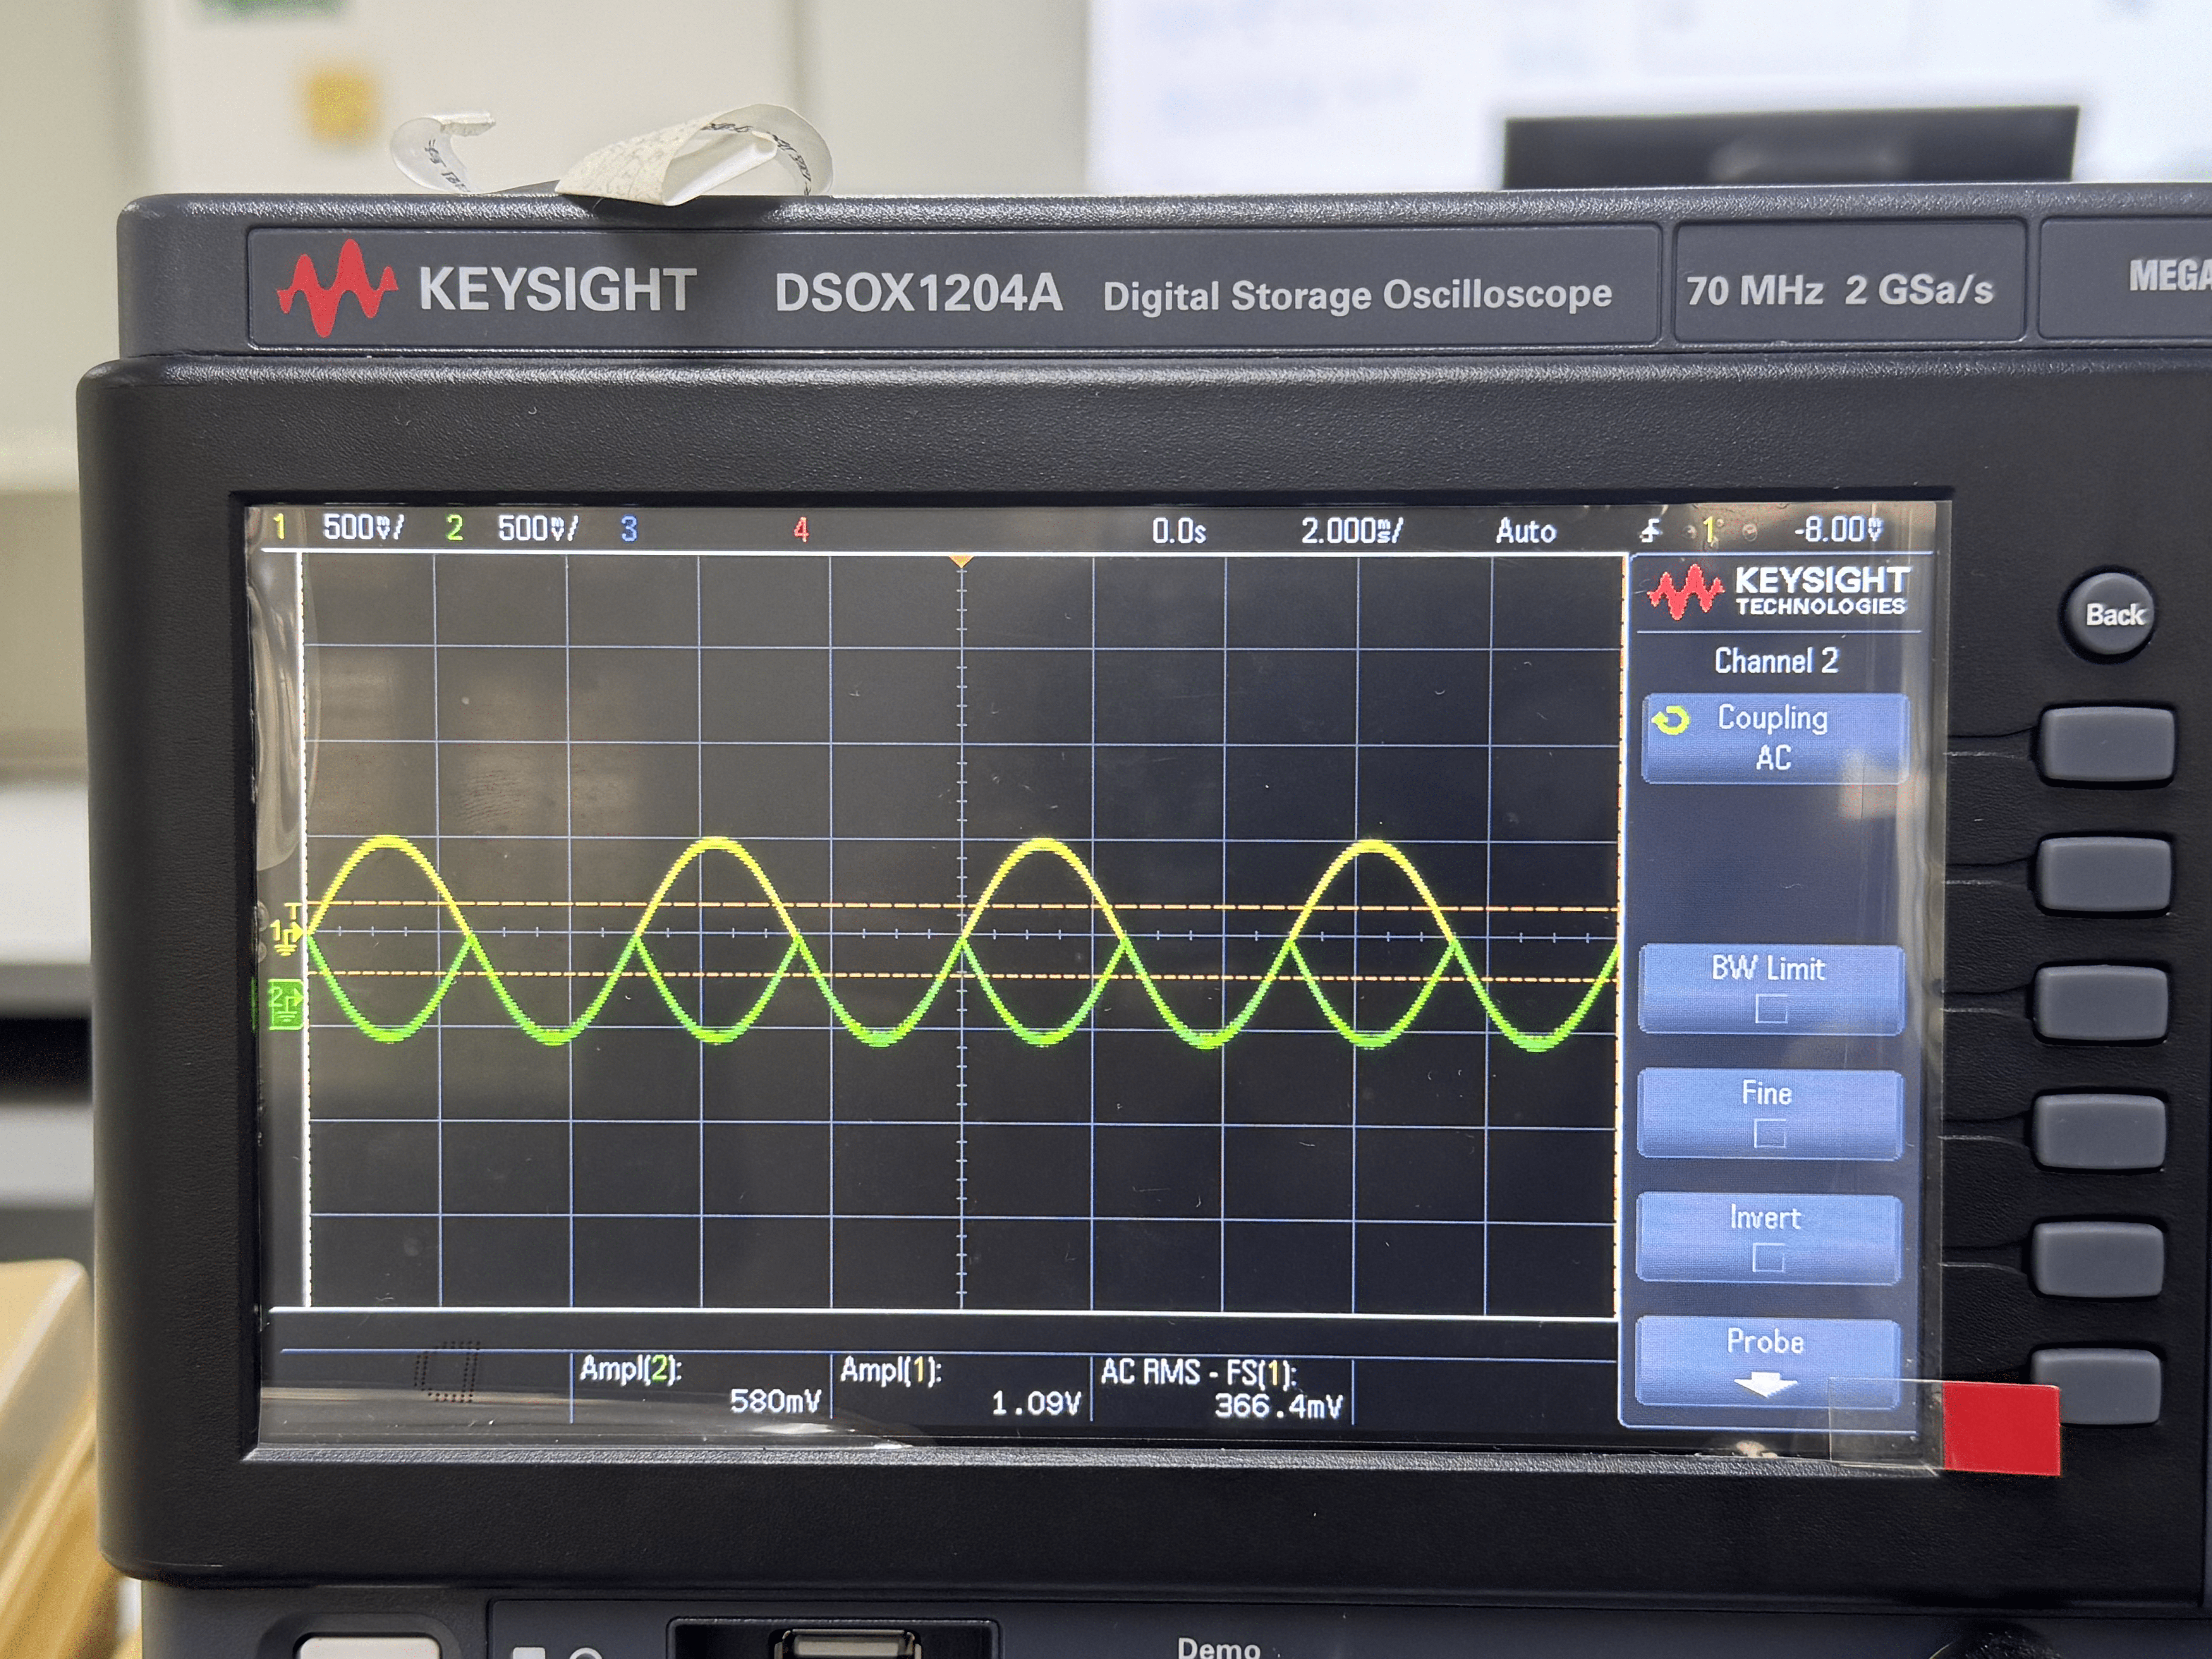
\includegraphics[width=0.5\linewidth]{Lab13/Images/13_5v.jpg}
            \caption{$V_i=5V$}
            \label{l13vi5v}
        \end{figure}
        \FloatBarrier
    From the figures above we can tell that all the positive signals are flipped into negative signals.\par
    And the amplitude of the input and the output signals are smaller than threshold voltage of the diodes.\par
    \subsubsection{DC}
    Let $V_i$ be a DC voltage signal, and measure the data with digital multi-meter.\\
        \begin{table}[h]
        \centering
            \begin{tabular}{|c|c|c|c|c|c|c|}
            \hline
            $V_i$ & -12    & -5     & -1     & 1       & 5       & 12      \\ \hline
            $V_1$ & -2.002 & 0      & 0      & 0       & 0       & 0       \\ \hline
            $V_2$ & 0      & 0      & 0      & 0       & 0       & 0       \\ \hline
            $V_3$ & 8.556  & 5.557  & 1.518  & -0.4965 & -0.5766 & -0.6254 \\ \hline
            $V_4$ & 7.913  & 4.953  & 0.9984 & -0.0011 & 0       & 0.4754  \\ \hline
            $V_5$ & -0.002 & -0.002 & -0.002 & -0.0018 & -0.0015 & 0.9517  \\ \hline
            $V_o$ & -4.143 & -5.131 & -1.029 & -1.013  & -5.045  & -9.211  \\ \hline
        \end{tabular}
        \end{table}
        \FloatBarrier
    When $V_i$ are taking -12, the most of measured values are not equal to theoretical relationships. It is because the $V_i$ is smaller than the supply voltages (-10), therefore the virtual short is not applied in this case (condition of output cannot be saturation is not met).
\section{Discussion}
    When we are calculating the theoretical values of the circuit related to Op.Amp., we need to consider the condition that whether the virtual short is applied in this case. In most of the time, the virtual open is applied, it can be used in the wide range of the cases, while the virtual short is depending on:\\
        \begin{itemize}
            \item whether there is negative feedback
            \item whether the output is in the range of $V^\pm$
        \end{itemize}

\section{Conclusion}
    In this chapter, we verified a precise full-wave rectifier. It is a rectifier specifically designed for small-signal circuit, because the traditional rectifiers using diodes have limitations due to the diode's forward voltage drop.\par
    A precise full-wave rectifier uses Op.Amp. to overcome the limitation of low voltage operation, ensuring that the rectification is accurate even for signals below the diode's threshold voltage.\par
    Overall, I learned more about the practical usage of Op.Amp. Moreover, the experiment enhances my knowledge of the Op.Amp. and the full-wave rectifier.